% 6.电路基础.tex 子文件，book文档类，主文档通过\input{6.电路基础.tex}导入
\chapter{第十章 二端口网络}

\section{二端口网络}

\section{导纳参数方程和阻抗参数方程}
\subsection{导纳参数方程}
如果二端口$Y$参数同时满足

代数方程
\[
\begin{cases}
\dot{I}_1 = Y_{11}\dot{U}_1 + Y_{12}\dot{U}_2 \\
\dot{I}_2 = Y_{21}\dot{U}_1 + Y_{22}\dot{U}_2
\end{cases}
\]

矩阵方程
\[
\begin{bmatrix}
\dot{I}_1 \\
\dot{I}_2
\end{bmatrix}
=
\begin{bmatrix}
Y_{11} & Y_{12} \\
Y_{21} & Y_{22}
\end{bmatrix}
\begin{bmatrix}
\dot{U}_1 \\
\dot{U}_2
\end{bmatrix}
\]

参数计算
\begin{align*}
Y_{11} &= \left. \frac{\dot{I}_1}{\dot{U}_1} \right|_{\dot{U}_2 = 0}\\
Y_{12} &= \left.  \frac{\dot{I}_1}{\dot{U}_2} \right|_{\dot{U}_1 = 0} \\
Y_{21} &= \left. \frac{\dot{I}_2}{\dot{U}_1} \right|_{\dot{U}_2 = 0}\\
Y_{22} &= \left. \frac{\dot{I}_2}{\dot{U}_2} \right|_{\dot{U}_1 = 0}
\end{align*}

互易对称条件：
\[
\text{互易： } Y_{12} = Y_{21},\quad
\text{对称： } Y_{12} = Y_{21} \text{，且 } Y_{11} = Y_{22}
\]

\subsection{阻抗参数方程}
代数方程
\[
\begin{cases}
\dot{U}_1 = Z_{11}\dot{I}_1 + Z_{12}\dot{I}_2 \\
\dot{U}_2 = Z_{21}\dot{I}_1 + Z_{22}\dot{I}_2
\end{cases}
\]

矩阵方程
\[
\begin{bmatrix}
\dot{U}_1 \\
\dot{U}_2
\end{bmatrix}
=
\begin{bmatrix}
Z_{11} & Z_{12} \\
Z_{21} & Z_{22}
\end{bmatrix}
\begin{bmatrix}
\dot{I}_1 \\
\dot{I}_2
\end{bmatrix}
\]

参数计算
\begin{align*}
Z_{11} &= \left. \frac{\dot{U}_1}{\dot{I}_1} \right|_{\dot{I}_2 = 0} \\
Z_{12} &= \left. \frac{\dot{U}_1}{\dot{I}_2} \right|_{\dot{I}_1 = 0} \\
Z_{21} &= \left. \frac{\dot{U}_2}{\dot{I}_1} \right|_{\dot{I}_2 = 0} \\
Z_{22} &= \left. \frac{\dot{U}_2}{\dot{I}_2} \right|_{\dot{I}_1 = 0}
\end{align*}

互易对称条件：
\[
\text{互易： } Z_{12} = Z_{21},\quad
\text{对称： } Z_{12} = Z_{21} \text{，且 } Z_{11} = Z_{22}
\]

\section{传输参数方程和混合参数方程}
\subsection{传输参数方程}
代数方程
\[
\begin{cases}
\dot{U}_1 = A_{11}\dot{U}_2 + A_{12}(-\dot{I}_2) \\
\dot{I}_1 = A_{21}\dot{U}_2 + A_{22}(-\dot{I}_2)
\end{cases}
\]

矩阵方程
\[
\begin{bmatrix}
\dot{U}_1 \\
\dot{I}_1
\end{bmatrix}
=
\begin{bmatrix}
A_{11} & A_{12} \\
A_{21} & A_{22}
\end{bmatrix}
\begin{bmatrix}
\dot{U}_2 \\
-\dot{I}_2
\end{bmatrix}
\]

参数计算
\begin{align*}
A_{11} &= \left. \frac{\dot{U}_1}{\dot{U}_2} \right|_{\dot{I}_2 = 0} \\
A_{21} &= \left. \frac{\dot{I}_1}{\dot{U}_2} \right|_{\dot{I}_2 = 0} \\
A_{12} &= \left. \frac{\dot{U}_1}{-\dot{I}_2} \right|_{\dot{U}_2 = 0} \\
A_{22} &= \left. \frac{\dot{I}_1}{-\dot{I}_2} \right|_{\dot{U}_2 = 0}
\end{align*}

互易对称条件：
\[
\text{互易： }A_{11}A_{22} - A_{12}A_{21} = 1,\quad
\text{对称： } A_{11}A_{22} - A_{12}A_{21} = 1 ,\text{且 } A_{11} = A_{22}
\]

将$Z$参数转换为$A$参数：
\[
A_{11}=\frac{Z_{11}}{Z_{21}},\;
A_{12}=\frac{Z_{11}Z_{22}-Z_{12}Z_{21}}{Z_{21}},\;
A_{21}=\frac{1}{Z_{21}},\;
A_{22}=\frac{Z_{22}}{Z_{21}}.
\]

\subsection{混合参数方程}
代数方程
\[
\begin{cases}
\dot{U}_1 = H_{11}\dot{I}_1 + H_{12}\dot{U}_2 \\
\dot{I}_2 = H_{21}\dot{I}_1 + H_{22}\dot{U}_2
\end{cases}
\]

矩阵方程
\[
\begin{bmatrix}
\dot{U}_1 \\
\dot{I}_2
\end{bmatrix}
=
\begin{bmatrix}
H_{11} & H_{12} \\
H_{21} & H_{22}
\end{bmatrix}
\begin{bmatrix}
\dot{I}_1 \\
\dot{U}_2
\end{bmatrix}
\]

参数计算
\begin{align*}
H_{11} &= \left. \frac{\dot{U}_1}{\dot{I}_1} \right|_{\dot{U}_2 = 0} \\
H_{21} &= \left. \frac{\dot{I}_2}{\dot{I}_1} \right|_{\dot{U}_2 = 0} \\
H_{12} &= \left. \frac{\dot{U}_1}{\dot{U}_2} \right|_{\dot{I}_1 = 0}\\
H_{22} &= \left. \frac{\dot{I}_2}{\dot{U}_2} \right|_{\dot{I}_1 = 0}
\end{align*}

互易对称条件：
\[
\text{互易: } H_{12} = -H_{21},\quad
\text{对称: } H_{12} = -H_{21},\text{ 且 } H_{11}H_{22} - H_{12}H_{21} = 1
\]

\section{二端口网络的等效电路}
如果给定
\[
Z_1=Z_{11}-Z_{12};\quad
Z_2=Z_{22}-Z_{21};\quad
Z_3=Z_{12}
\]
上式应与。

如果二端口网络给定的是$Y$参数，则宜选用$\varPi$形等效电路，以便
\[
Y_1=Y_{11}+Y_{12};\quad
Y_3=-Y_{21}=-Y_{12};\quad
Y_2=Y_{22}+Y_{21}
\]

如果，得
\[
Z_1=\frac{A_{11}-1}{A_{21}};\quad
Z_2=\frac{A_{22}-1}{A_{21}};\quad
Z_3=\frac{1}{A_{21}}
\]
\[
Y_a=\frac{A_{22}-1}{A_{12}};\quad
Y_b=\frac{A_{11}-1}{A_{12}};\quad
Y_c=\frac{1}{A_{12}}
\]

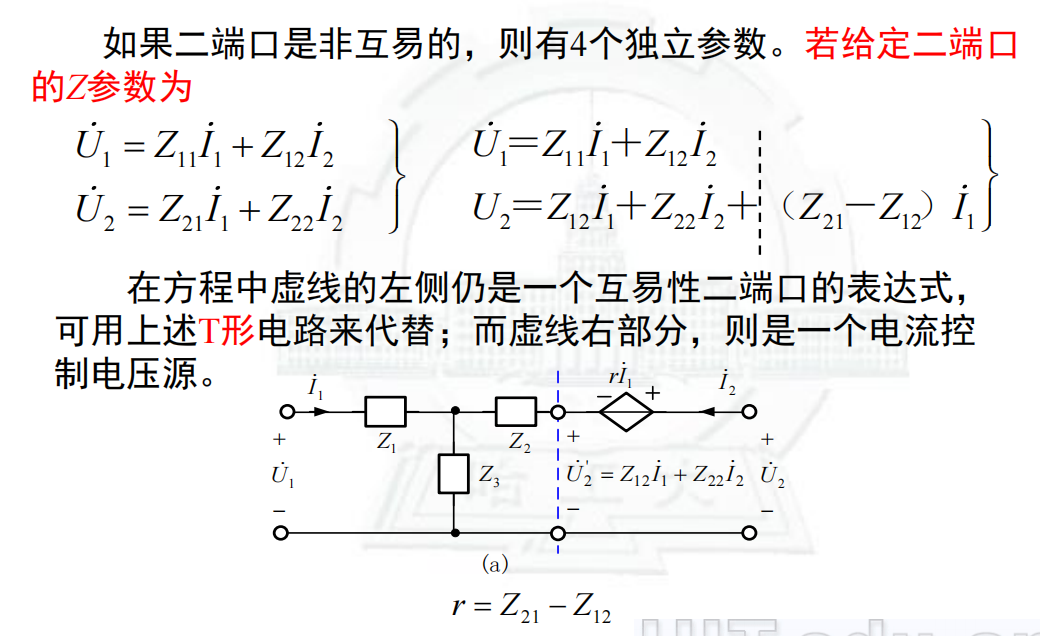
\includegraphics[width=0.6\textwidth]{10.4.1.png}\par
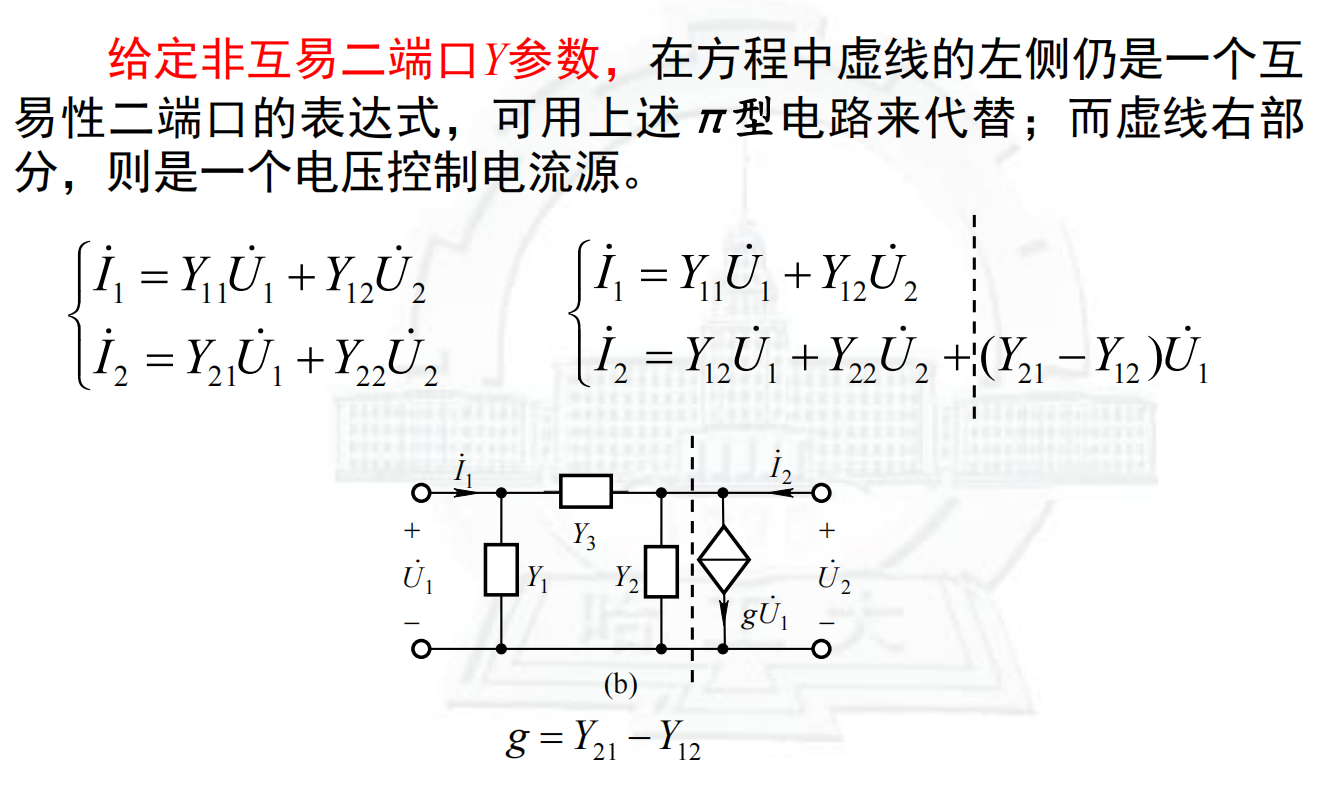
\includegraphics[width=0.6\textwidth]{10.4.2.png}\par

\section{二端口网络与电源和负载的连接}
\subsection{输入阻抗、输出阻抗}
输入阻抗。

特性阻抗（不做要求）。

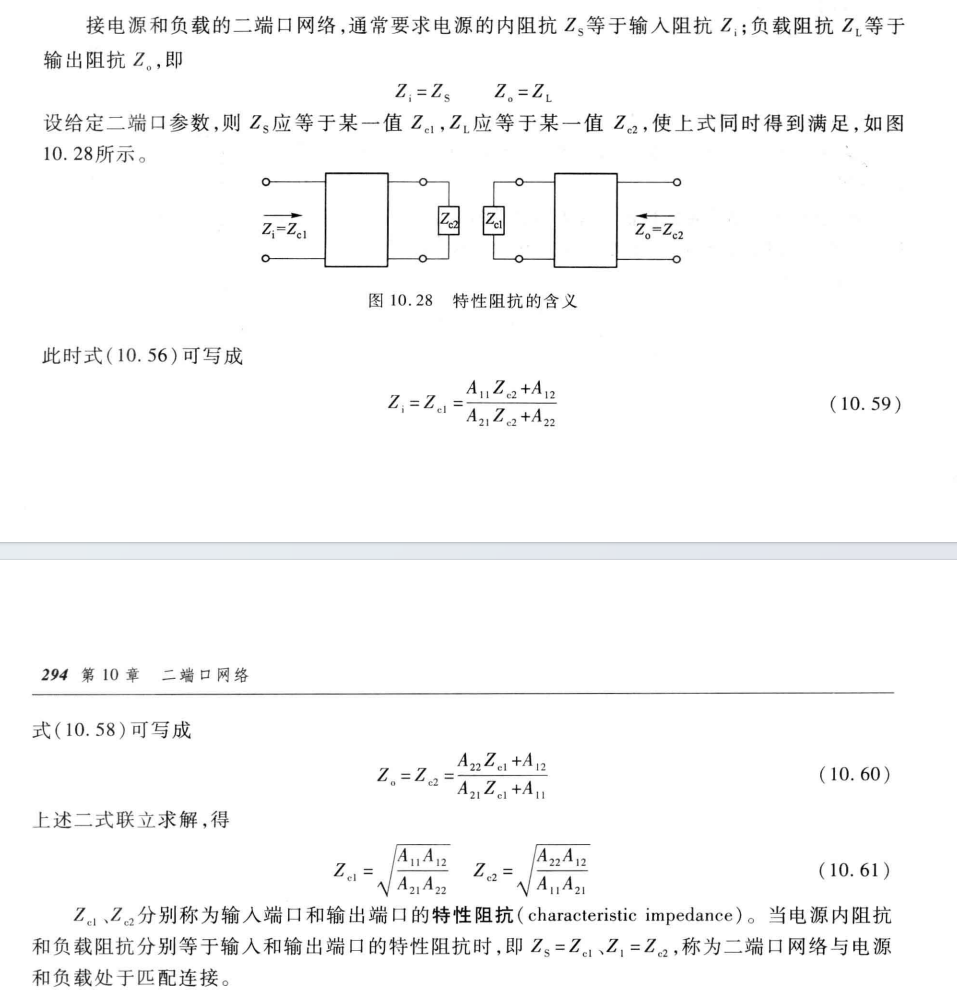
\includegraphics[width=0.6\textwidth]{10.3.png}\par

对称二端口网络的传输系数和特性阻抗。

\section{二端口网络的级联}

\endinput
